\documentclass{standalone}

\usepackage{tikz}
\usepackage{circuitikz}

\tikzset{block/.style = {draw, fill=white, very thick, rectangle, minimum height=1cm, minimum width=2cm},
         lblock/.style={draw,fill=white,very thick, rectangle, minimum height=3cm, minimum width=1cm},
         sum/.style= {draw, fill=white, very thick, circle, node distance=0.5cm}}

         
\begin{document}
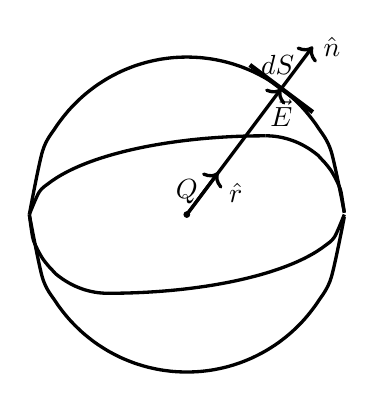
\begin{tikzpicture}[scale=2]
    \draw[-, very thick]plot[smooth, domain=-1:1](\x, {(1-(\x)^2)^0.5});
    \draw[-, very thick]plot[smooth, domain=-1:1](\x, {-(1-(\x)^2)^0.5});
    \draw[-, very thick]plot[smooth, domain=0.5:1](\x,{(0.25-(\x-0.5)^2)^0.5});
    \draw[-, very thick]plot[smooth, domain=-1:-0.5](\x,{-(0.25-(\x+0.5)^2)^0.5});
    \draw[-, very thick]plot[smooth, domain=-1:0.5](\x,{1/3*(2.25-(\x-0.5)^2)^0.5});
    \draw[-, very thick]plot[smooth, domain=-0.5:1](\x,{-1/3*(2.25-(\x+0.5)^2)^0.5});

    \filldraw[black](0,0)circle(0.5pt);

    \draw[->, very thick](0,0)node[above]{$Q$}--(0.6,0.8)node[below]{$\vec{E}$};
    \draw[->,very thick](0,0)--(0.2,0.267)node[below right]{$\hat{r}$};

    \draw[-, ultra thick](0.4,0.95)node[right]{$dS$}--(0.8,0.65);
    \draw[->,very thick](0.6,0.8)--(0.8,1.067)node[right]{$\hat{n}$};
\end{tikzpicture}
\end{document}